\chapter{Лабораторная работа №6. Цифровая обработка сигналов}

\section{Арифметика с плавающей точкой}

\begin{figure}[h]
	\centering
	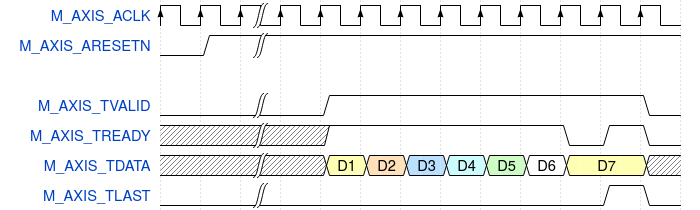
\includegraphics[width=0.9\textwidth]{image/axis_0.png}
	\caption{Временная диаграмма работы интерфейса AXI4-Stream}
	\label{axis}
\end{figure}

AXI4-Stream — это протокол, предназначенный для передачи однонаправленных данных(см.рис.~\ref{axis}). В AXI4-Stream биты ширины TDATA передаются за такт. Передача начинается, когда ведущее устройство(master) отправляет сигнал TVALID, а ведомое устройство(slave) отвечает, отправляя сигнал TREADY(этот механизм был рассмотрен выше, при рассмотрении интерфейса AXI4-Lite). В этот момент мастер начнет отправлять TDATA и TLAST (TUSER, если необходимо передать дополнительные данные, определяемые пользователем). TLAST сигнализирует о последнем слове потока. Таким образом, ведомое устройство(slave) продолжает потреблять входящие TDATA до тех пор, пока TLAST не будет установлен.

\begin{figure}[h]
	\centering
	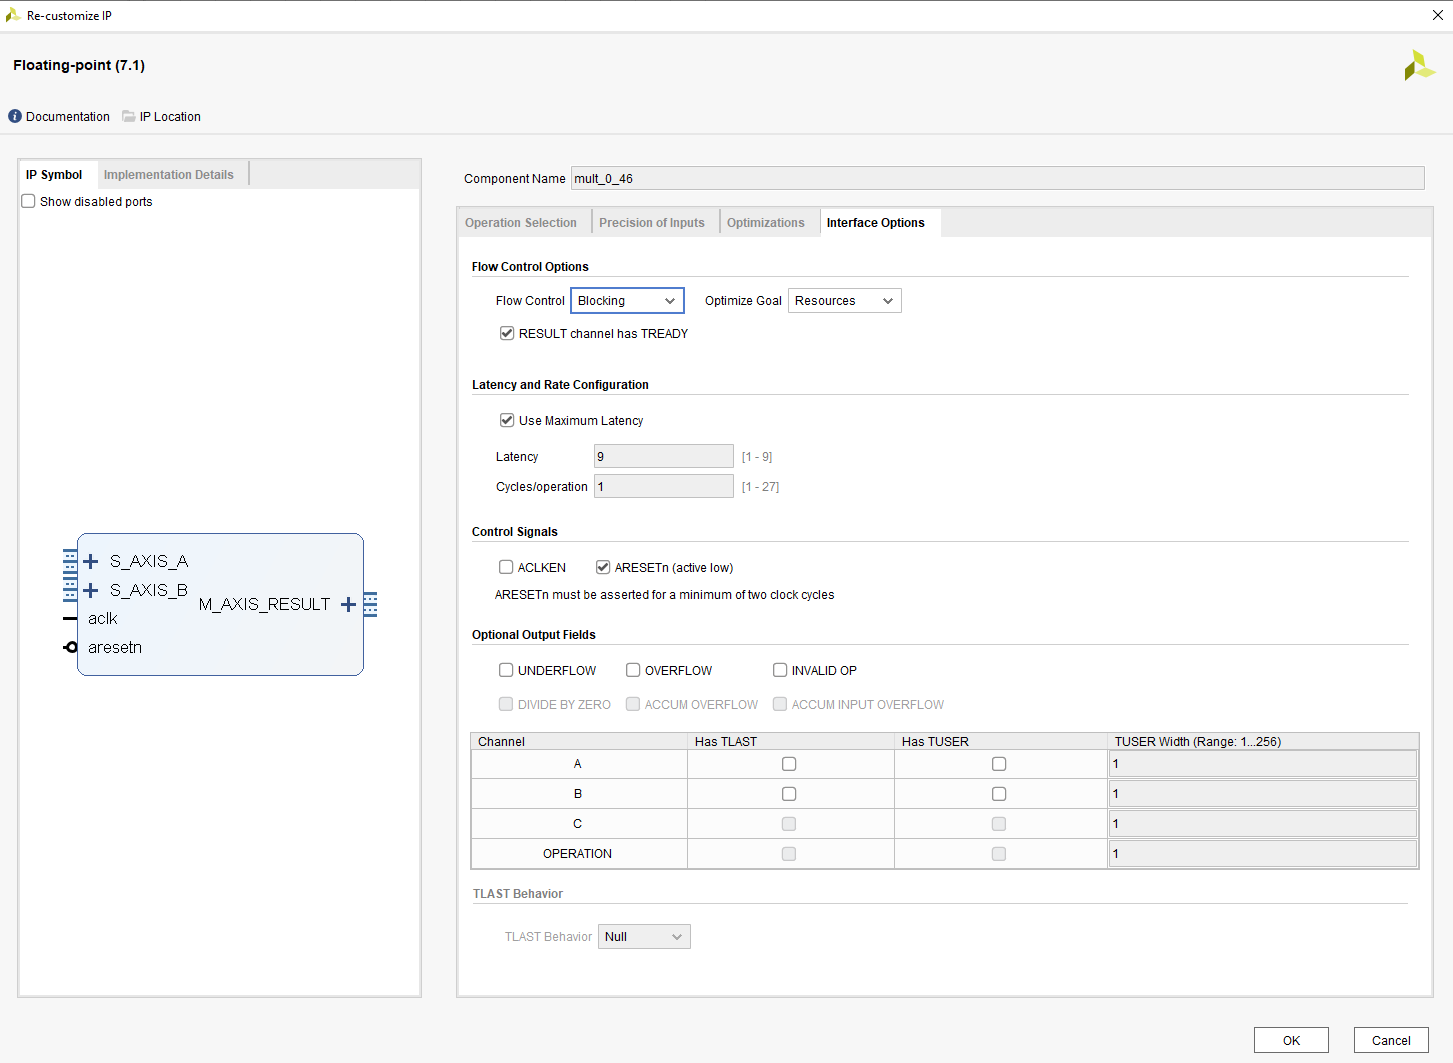
\includegraphics[width=0.5\textwidth]{image/fp_interface_options.png}
	\caption{Временная диаграмма работы интерфейса AXI4-Stream}
	\label{fp_interface_options}
\end{figure}

\begin{figure}[h]
	\centering
	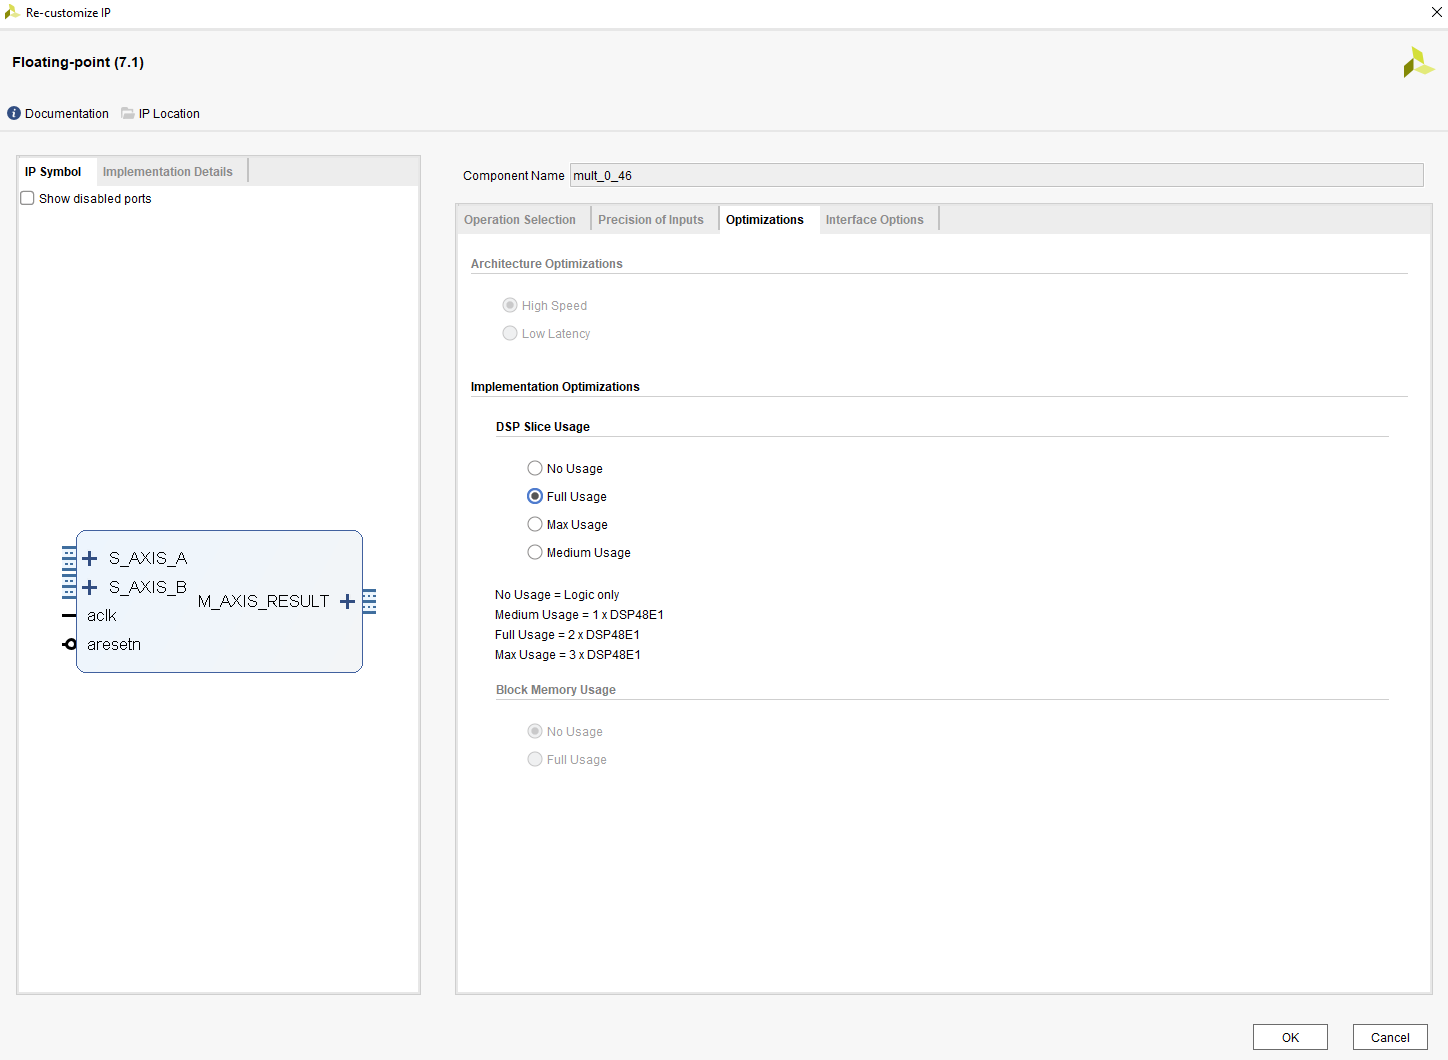
\includegraphics[width=0.5\textwidth]{image/fp_optimizations.png}
	\caption{Временная диаграмма работы интерфейса AXI4-Stream}
	\label{fp_optimizations}
\end{figure}

\begin{figure}[h]
	\centering
	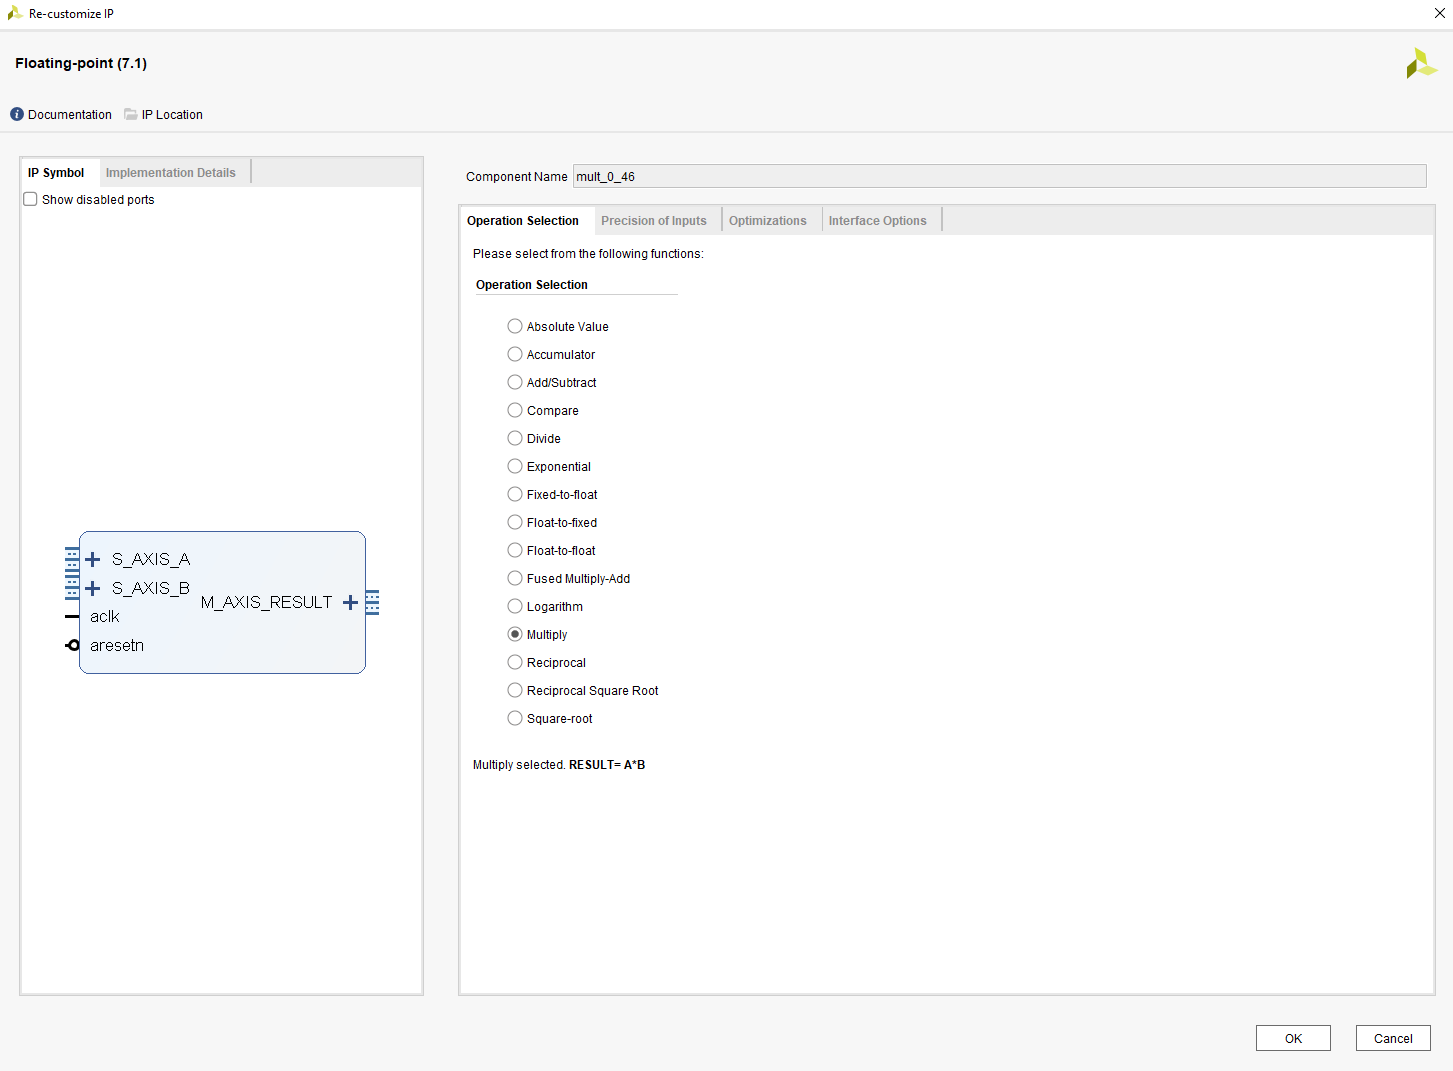
\includegraphics[width=0.5\textwidth]{image/fp_selection_tab.png}
	\caption{Временная диаграмма работы интерфейса AXI4-Stream}
	\label{fp_selection_tab}
\end{figure}

\begin{figure}[h]
	\centering
	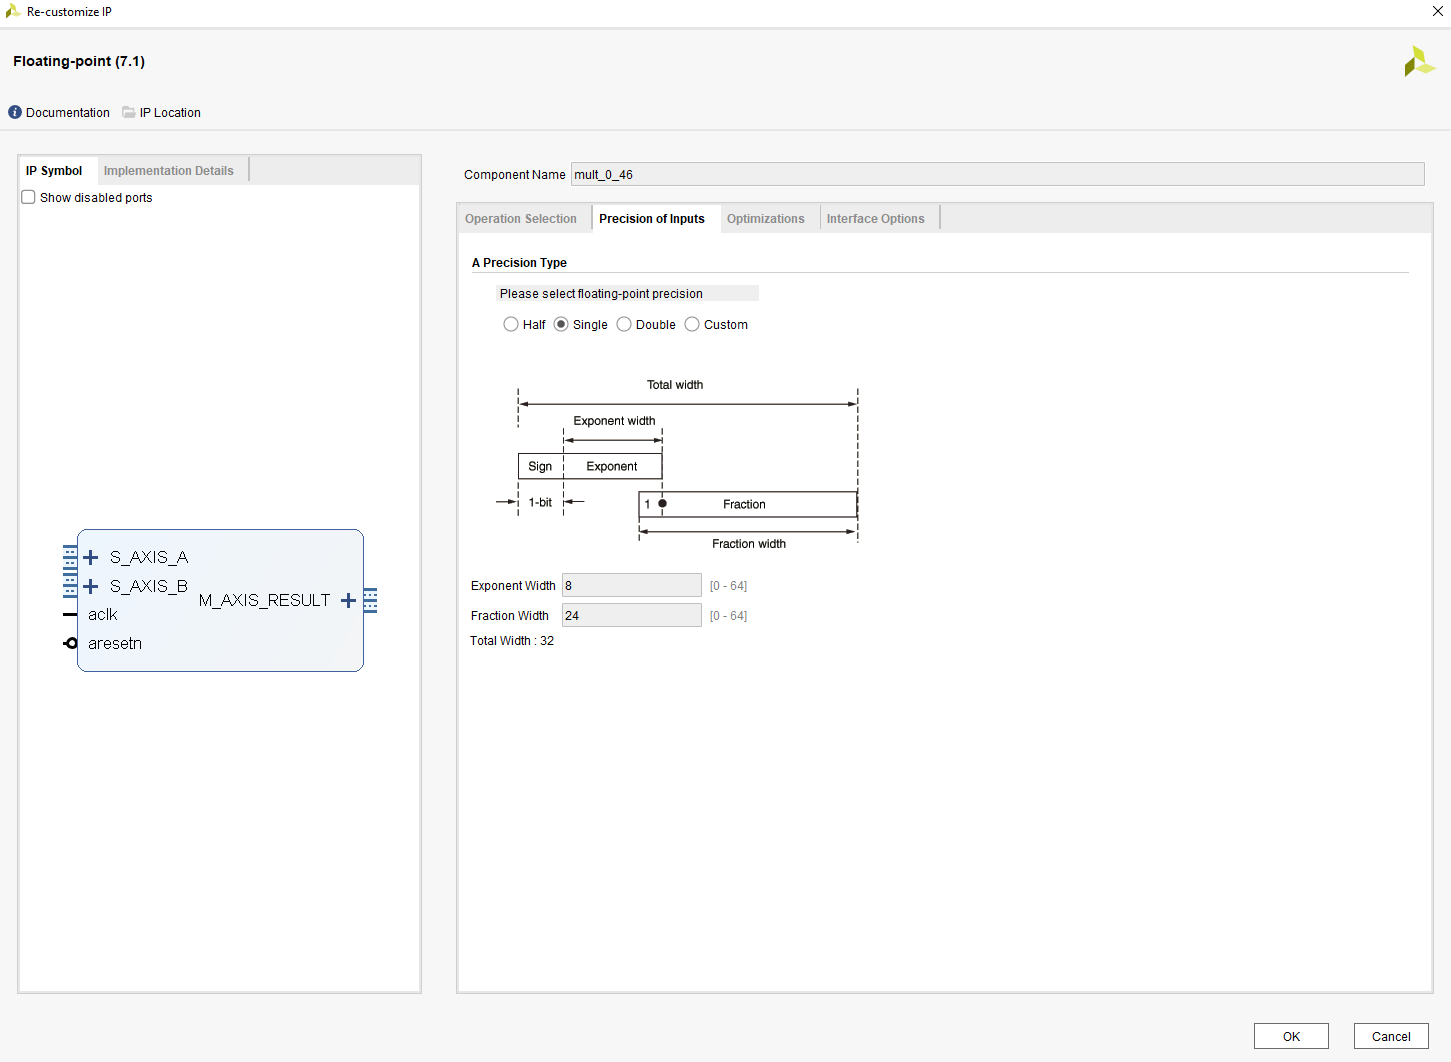
\includegraphics[width=0.5\textwidth]{image/fp_precision_type.png}
	\caption{Временная диаграмма работы интерфейса AXI4-Stream}
	\label{fp_precision_type}
\end{figure}

\section{Быстрое преобразование Фурье}
	Выражение для дискретного преобразования Фурье имеет следующий вид:

\begin{align*}
f[k] &= \sum_{j=0}^{N-1} x[j]\left(e^{-2\pi i k/N}\right)^j\\
0 &\leq k < N
\end{align*}

\begin{figure}[h]
    \centering
    \noindent
	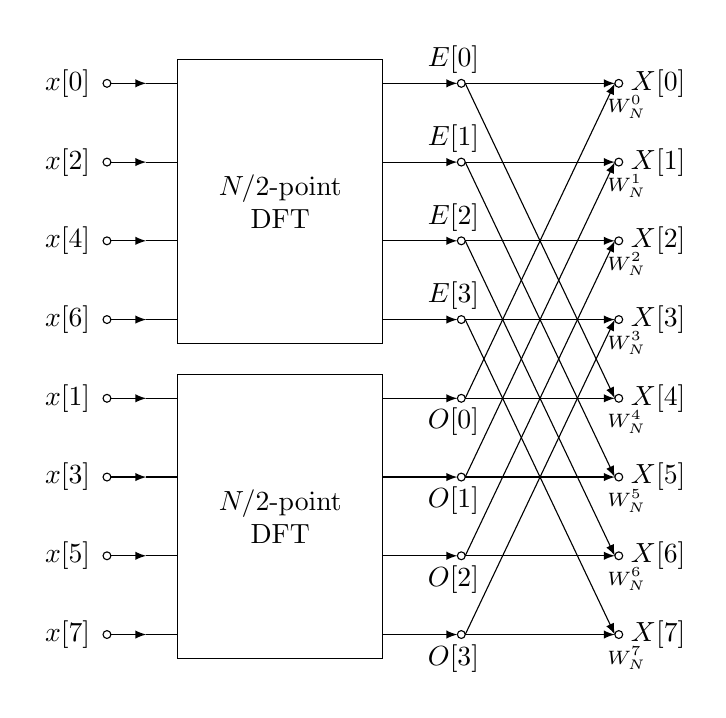
\begin{tikzpicture}% Example:
	  \draw[fill=white, draw=white] (-0.5, 0.7) rectangle (8, -7.7); 
	  \draw (0,0) node {$x[0]$};
	  \draw (0,-1) node {$x[2]$} ;
	  \draw (0,-2) node {$x[4]$} ;
	  \draw (0,-3) node {$x[6]$} ;
	
	  \draw (0,-4) node {$x[1]$} ;
	  \draw (0,-5) node {$x[3]$} ;
	  \draw (0,-6) node {$x[5]$} ;
	  \draw (0,-7) node {$x[7]$} ;
	
	  % arrow on the right of x's
	  \foreach \n in {0,...,7} {
	    \draw (0.5,-\n) circle(0.05)[fill=white]; 
	    \draw [-latex] (0.55,-\n) -- (1, -\n); 
	    \draw (1, -\n) -- (1.4, -\n); 
	  }
	
	  % blocks
	  \draw(1.4, 0.3) rectangle (4, -3.3); 
	  \draw(1.4, -3.7) rectangle (4, -7.3); 
	  \draw(2.7, -1.5) node[text centered, text width=2cm] {$N/2$-point DFT};
	  \draw(2.7, -5.5) node[text centered, text width=2cm] {$N/2$-point DFT};
	
	  % E's and O's 
	  \foreach \n in {0,...,7} {
	    \draw [-latex] (4,-\n) -- (4.95, -\n); 
	    \draw (5,-\n) circle(0.05)[fill=white]; 
	  }
	  \foreach \n in {0,...,3} {
	    \draw (4.9,-\n + 0.3) node {$E[\n]$};
	  }
	  \foreach \n in {0,...,3} {
	    \draw (4.9,-\n - 4 - 0.3) node {$O[\n]$};
	  }
	
	  % X's 
	  \foreach \n in {0,...,7} {
	    \draw (7,-\n) circle(0.05)[fill=white]; 
	    \draw (7.5,-\n) node {$X[\n]$};
	  }
	
	  % Connecting X and E
	  \foreach \n in {0,...,7} {
	    \draw [-latex] (5.05, -\n) -- (6.95, -\n);
	  }
	  \foreach \n in {0,...,3} {
	    \draw [-latex] (5.05, -\n) -- (6.95, -\n - 4);
	  }
	  \foreach \n in {0,...,3} {
	    \draw [-latex] (5.05, -\n-4) -- (6.95, -\n);
	  }
	
	  % W's
	  \foreach \n in {0,...,7} {
	    \draw (7.1,-\n - 0.3) node {\scriptsize $W_N^{\n}$};
	  }
	\end{tikzpicture}
\end{figure}

\begin{figure}[h]
	\centering
	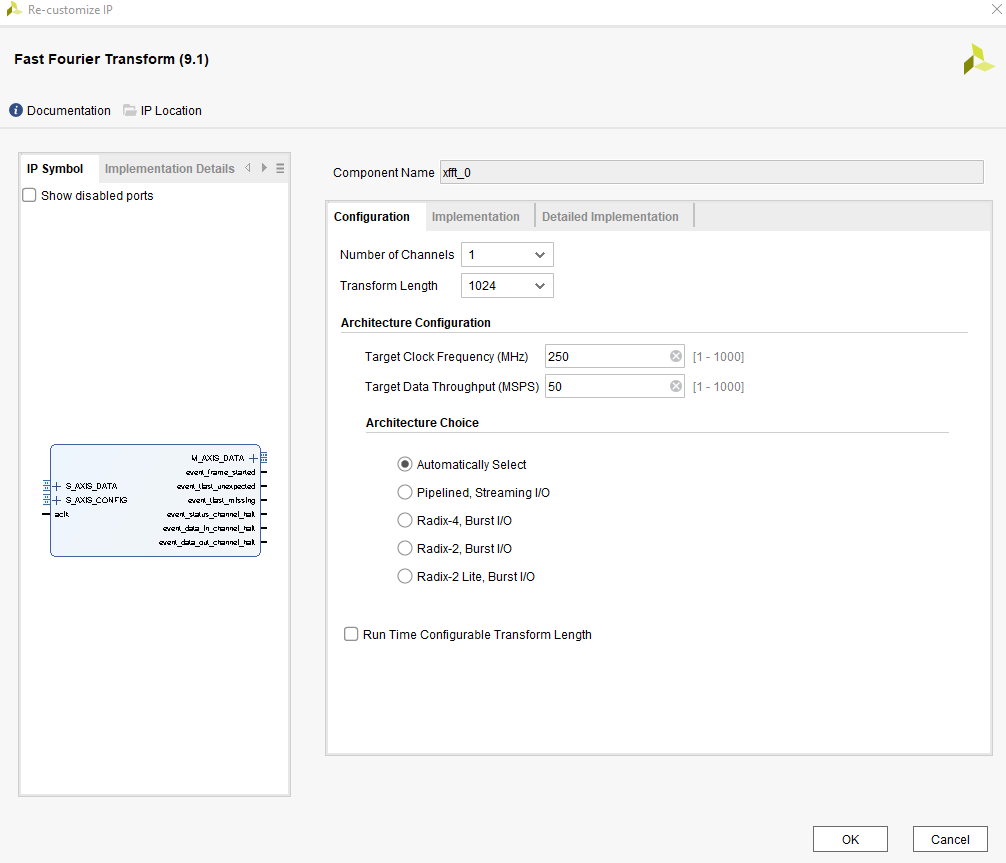
\includegraphics[width=0.5\textwidth]{image/fft_config.png}
	\caption{Временная диаграмма работы интерфейса AXI4-Stream}
	\label{fft_config}
\end{figure}
	
\begin{figure}[h]
	\centering
	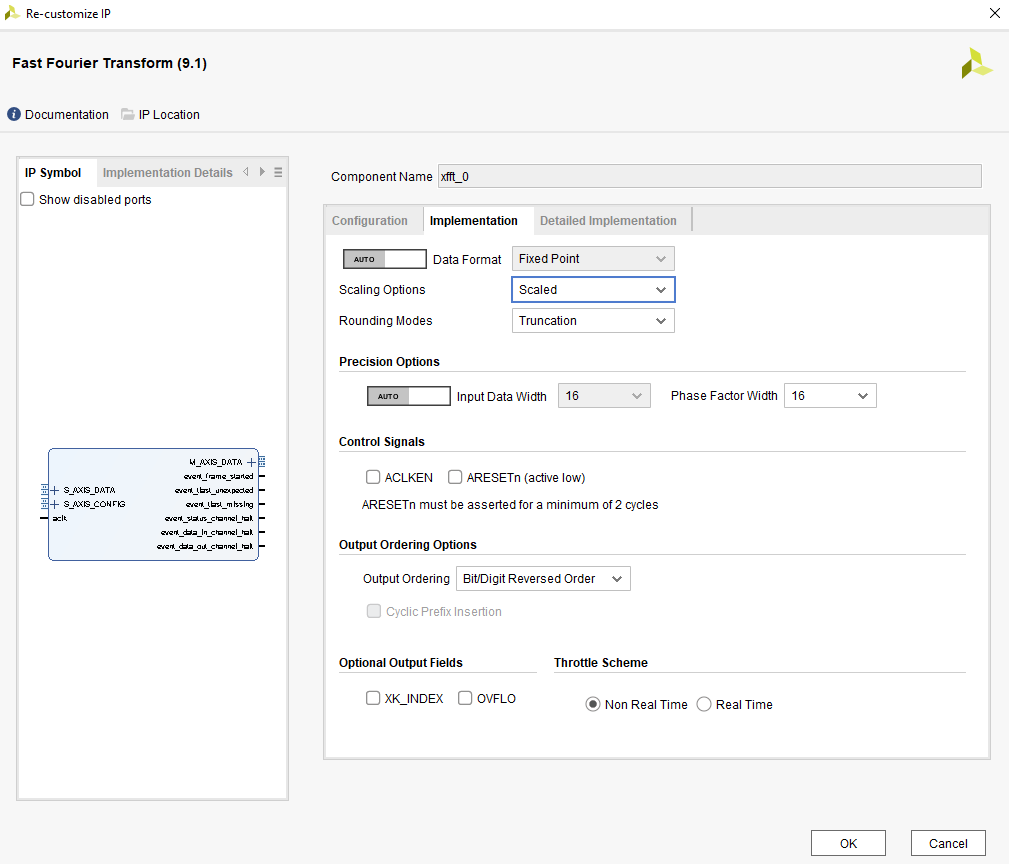
\includegraphics[width=0.5\textwidth]{image/fft_implemetation.png}
	\caption{Временная диаграмма работы интерфейса AXI4-Stream}
	\label{fft_implemetation}
\end{figure}
	
\begin{figure}[h]
	\centering
	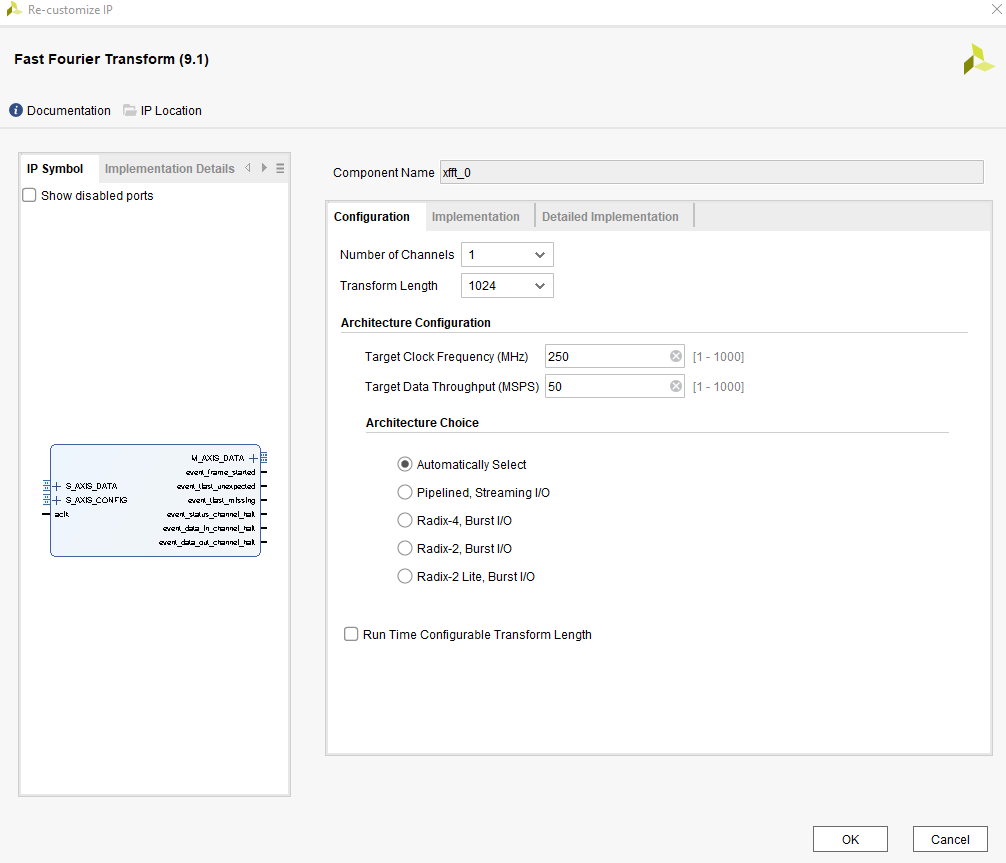
\includegraphics[width=0.5\textwidth]{image/fft_config.png}
	\caption{Временная диаграмма работы интерфейса AXI4-Stream}
	\label{fft_detailed_implem}
\end{figure}
	
\section{Сигнал с линейной-частотной модуляцией}

Сигнал с линейной-частотной модуляцией определяется по следующей формуле:
\begin{equation}	
	s(t) = rect(\frac{t}{T}) \cdot \cos(2 \cdot \pi \cdot f_0 \cdot t + j \cdot \pi \cdot K \cdot t^{2}),
\end{equation}

где t - время в секундах, K-скорость изменения частоты во времени, T - длительность импульса, rect() - прямоугольное окно, \(f_0\) - несущая частота.

После прохождения через квадратурный демодулятор получаем следующий комплексный сигнал:

\begin{equation}	
	g(t) = rect(\frac{t}{T}) \cdot \exp(j \cdot \pi \cdot K \cdot t^{2})
\end{equation}

Действительная часть называется квадратурной
составляющей ЛЧМ-сигнал, и обозначается как \(Q(t)\), а мнимая 
синфазной составляющей ЛЧМ-сигнала, и обозначается как \(I(t)\):

\begin{equation}	
	Q(t) = rect(\frac{t}{T}) \cdot \cos(\pi \cdot K \cdot t^{2}),
\end{equation}

\begin{equation}	
	I(t) = rect(\frac{t}{T}) \cdot \sin(\pi \cdot K \cdot t^{2}).
\end{equation}

Важнейшими параметрами ЛЧМ-сигнала являются:

\begin{enumerate}
	\item Девиация частоты: 
\begin{equation}
	BW = |K| \cdot T, 
\end{equation}
измеряется в Гц.
	\item База: 
\begin{equation}
	B = |K| \cdot T^2, 
\end{equation}
безразмерная величина.
\end{enumerate}

Рассмотрим конкретный пример демодулированного ЛЧМ-сигнала. Пусть он имеет следующие параметры: частота дискретизации \(F_{D}\) = 1000 МГц, девиация частоты \(BW\) = 400 МГц, длительность сигнала \(T\) = 4 мкс. На рисунке ~\ref{fig:chirp_q} представлена квадратурная составляющая ЛЧМ-сигнала с приведёнными выше параметрами, а на рисунке ~\ref{fig:chirp_i} представлена синфазная составляющая ЛЧМ-сигнала с приведёнными выше параметрами.

\begin{figure}[h]
    \centering
    \noindent
    \begin{tikzpicture}
        \begin{axis}
            [
            RCS Plot,
            title={},
            height=0.4\textwidth,
            xlabel={Время, мкс},
            ylabel={Амплитуда, отсчётов},
            legend pos = south east
            ]
            \addplot table {Synopsis/data/third-party/lfm_im.dat};
            \addlegendentry{Q(t)};
            \addplot table {Synopsis/data/third-party/lfm_re.dat};
            \addlegendentry{I(t)};
        \end{axis}
    \end{tikzpicture}
    \caption{Квадратурная составляющая ЛЧМ сигнала}
    \label{fig:chirp_q}
\end{figure}

\begin{figure}[h]
    \centering
    \noindent
    \begin{tikzpicture}
        \begin{axis}
            [
            RCS Plot,
            title={},
            height=0.4\textwidth,
            xlabel={Время, мкс},
            ylabel={Амплитуда, отсчётов},
            legend pos = south east
            ]
            \addplot table {Synopsis/data/third-party/lfm_shift_im.dat};
            \addlegendentry{Q(t)};
            \addplot table {Synopsis/data/third-party/lfm_shift_re.dat};
            \addlegendentry{I(t)};
        \end{axis}
    \end{tikzpicture}
    \caption{Квадратурная составляющая ЛЧМ сигнала}
    \label{fig:chirp_q}
\end{figure}

\begin{figure}[h]
    \centering
    \noindent
    \begin{tikzpicture}
        \begin{axis}
            [
            RCS Plot,
            title={},
            height=0.4\textwidth,
            xlabel={Время, мкс},
            ylabel={Амплитуда, отсчётов},
            legend pos = south east
            ]
            \addplot table {Synopsis/data/third-party/lfm_shift_noise_im.dat};
            \addlegendentry{Q(t)};
            \addplot table {Synopsis/data/third-party/lfm_shift_noise_re.dat};
            \addlegendentry{I(t)};
        \end{axis}
    \end{tikzpicture}
    \caption{Квадратурная составляющая ЛЧМ сигнала}
    \label{fig:chirp_q}
\end{figure}

\begin{figure}[h]
    \centering
    \noindent
    \begin{tikzpicture}
        \begin{axis}
            [
            RCS Plot,
            title={},
            height=0.4\textwidth,
            xlabel={Время, мкс},
            ylabel={Амплитуда, отсчётов},
            legend pos = south east
            ]
            \addplot table {Synopsis/data/third-party/correl_re.dat};
            \addlegendentry{I(t)};
			\addplot table {Synopsis/data/third-party/correl_im.dat};
            \addlegendentry{I(t)};
        \end{axis}
    \end{tikzpicture}
    \caption{Синфазная составляющая ЛЧМ сигнала}
    \label{fig:chirp_i}
\end{figure}


\begin{figure}[h]
	\centering
	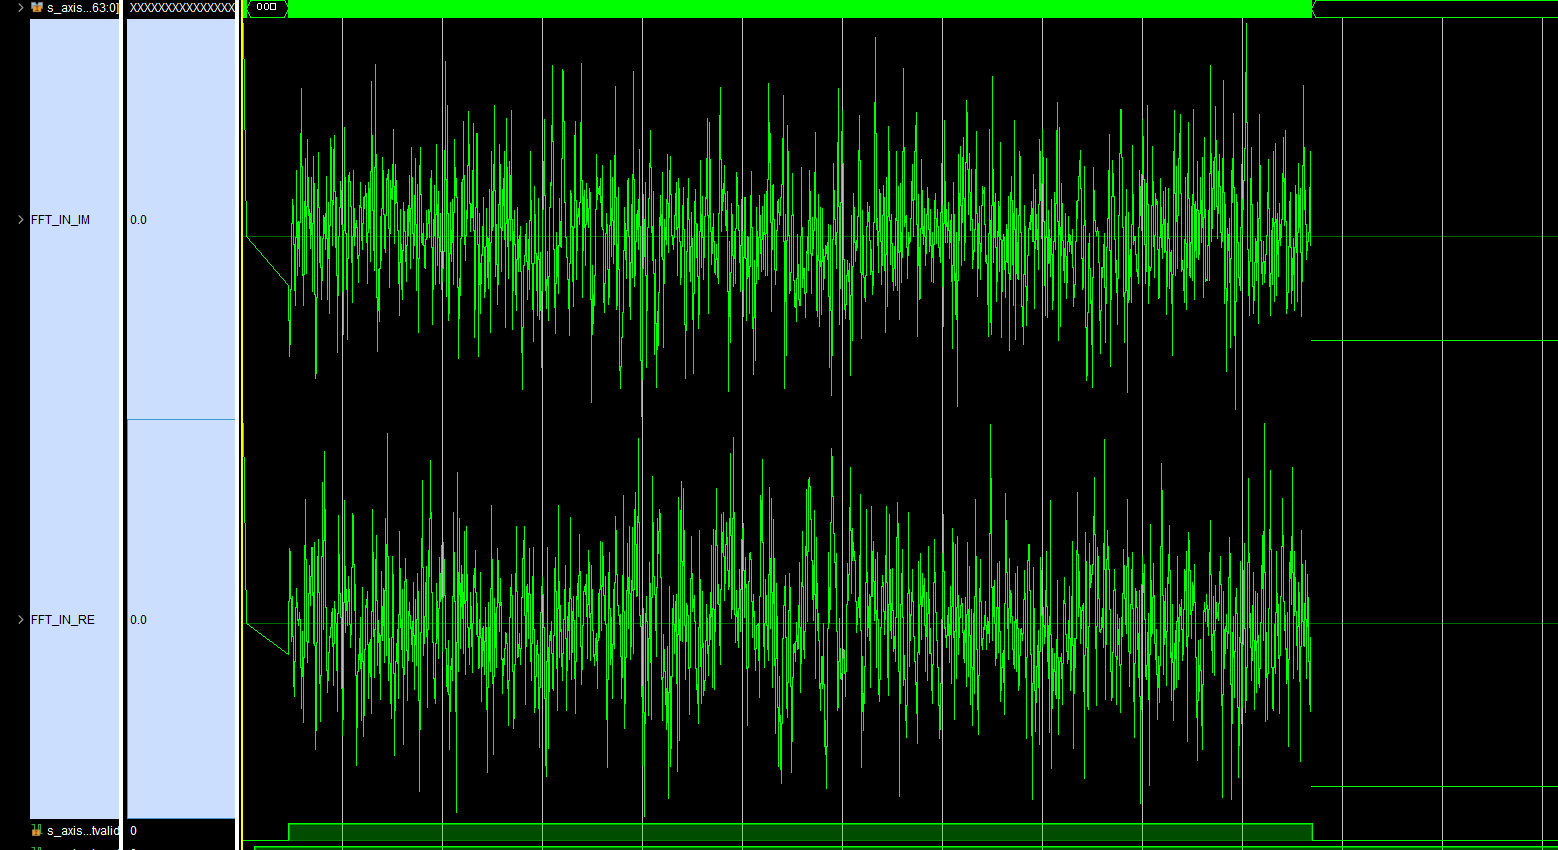
\includegraphics[width=0.5\textwidth]{image/lfm_with_noise.png}
	\caption{Временная диаграмма работы интерфейса AXI4-Stream}
	\label{fft_result}
\end{figure}
	
\begin{figure}[h]
	\centering
	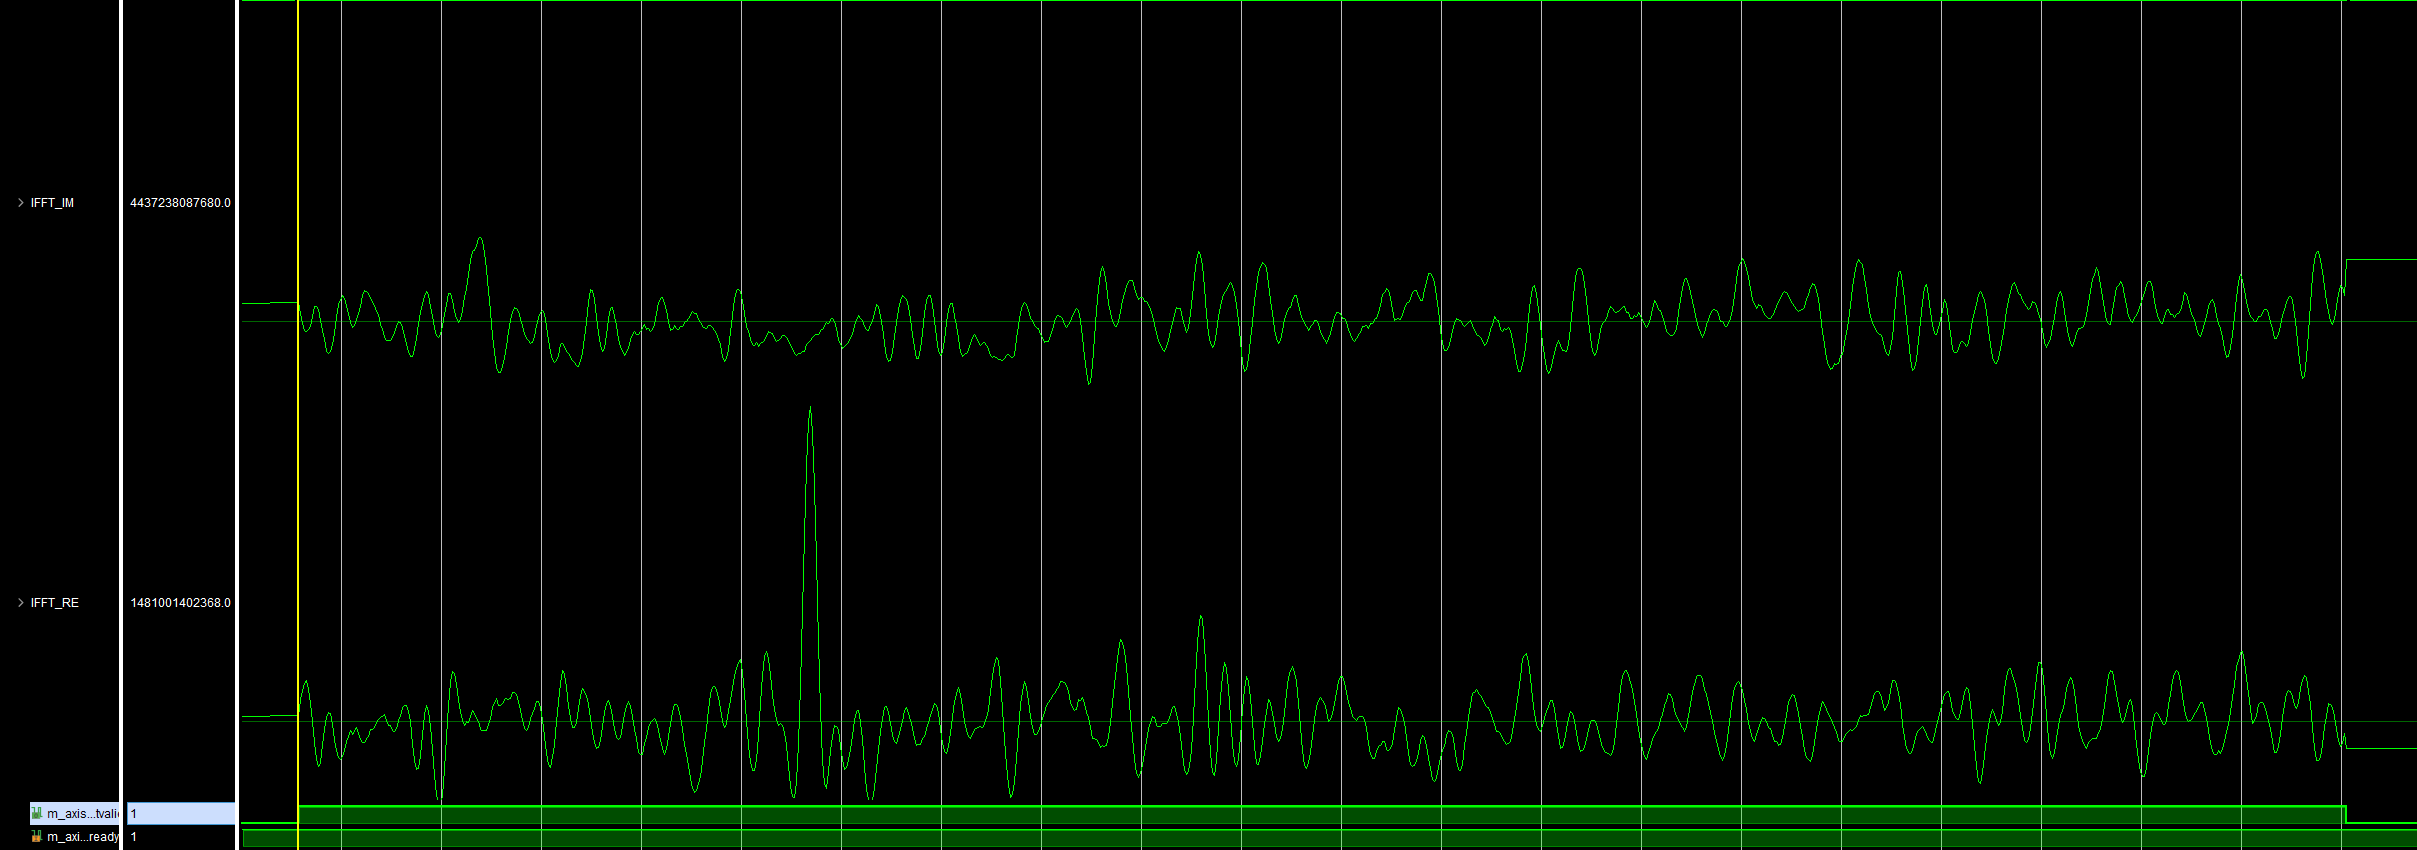
\includegraphics[width=0.5\textwidth]{image/correl_with_noise.png}
	\caption{Временная диаграмма работы интерфейса AXI4-Stream}
	\label{fft_detailed_implem}
\end{figure}

\section{Практическая часть}


